\documentclass[aspectratio=43,english]{beamer} %If you want to create Polish presentation, replace 'english' with 'polish' and uncomment 3-th line, i.e., '\usepackage{polski}'
\usepackage[utf8]{inputenc}
\usepackage{polski} %Uncomment for Polish language
\usepackage{babel}
\usepackage{listings} %We want to put listings

\mode<beamer>{ 	%in 'beamer' mode
	\hypersetup{pdfpagemode=FullScreen}		%Enable Full screen mode
	\usetheme{JuanLesPins} 		%Show part title in right footer
	%\usetheme[dark]{AGH}                 		%Use dark background
	%\usetheme[dark,parttitle=leftfooter]{AGH}  	%Use dark background and show part title in left footer
}
\mode<handout>{	%in 'handout' mode
	\hypersetup{pdfpagemode=None}		
	\usepackage{pgfpages}
  	\pgfpagesuselayout{4 on 1}[a4paper,border shrink=5mm,landscape]	%show 4 slides on 1 page
  	\usetheme{boxes}
  	\addheadbox{structure}{\quad\insertpart\hfill\insertsection\hfill\insertsubsection\qquad} 	%content of header
 	\addfootbox{structure}{\quad\insertauthor\hfill\insertframenumber\hfill\insertsubtitle\qquad} 	%content of footer
}

\AtBeginPart{ %At begin part: display its name
	\frame{\partpage}
} 


%%%%%%%%%%% Configuration of the listings package %%%%%%%%%%%%%%%%%%%%%%%%%%
% Source: https://en.wikibooks.org/wiki/LaTeX/Source_Code_Listings#Using_the_listings_package
%%%%%%%%%%%%%%%%%%%%%%%%%%%%%%%%%%%%%%%%%%%%%%%%%%%%%%%%%%%%%%%%%%%%%%%%%%%%
\lstset{ %
  backgroundcolor=\color{white},   % choose the background color
  basicstyle=\footnotesize,        % the size of the fonts that are used for the code
  breakatwhitespace=false,         % sets if automatic breaks should only happen at whitespace
  breaklines=true,                 % sets automatic line breaking
  captionpos=b,                    % sets the caption-position to bottom
  commentstyle=\color{green},      % comment style
  deletekeywords={...},            % if you want to delete keywords from the given language
  escapeinside={\%*}{*)},          % if you want to add LaTeX within your code
  extendedchars=true,              % lets you use non-ASCII characters; for 8-bits encodings only, does not work with UTF-8
  frame=single,	                   % adds a frame around the code
  keepspaces=true,                 % keeps spaces in text, useful for keeping indentation of code (possibly needs columns=flexible)
  keywordstyle=\color{blue},       % keyword style
  morekeywords={*,...},            % if you want to add more keywords to the set
  numbers=left,                    % where to put the line-numbers; possible values are (none, left, right)
  numbersep=5pt,                   % how far the line-numbers are from the code
  numberstyle=\tiny\color{gray},   % the style that is used for the line-numbers
  rulecolor=\color{black},         % if not set, the frame-color may be changed on line-breaks within not-black text (e.g. comments (green here))
  showspaces=false,                % show spaces everywhere adding particular underscores; it overrides 'showstringspaces'
  showstringspaces=false,          % underline spaces within strings only
  showtabs=false,                  % show tabs within strings adding particular underscores
  stepnumber=2,                    % the step between two line-numbers. If it's 1, each line will be numbered
  stringstyle=\color{cyan},        % string literal style
  tabsize=2,	                   % sets default tabsize to 2 spaces
  title=\lstname,                  % show the filename of files included with \lstinputlisting; also try caption instead of title
                                   % needed if you want to use UTF-8 Polish chars
  literate={?}{{\k{a}}}1
           {?}{{\k{A}}}1
           {?}{{\k{e}}}1
           {?}{{\k{E}}}1
           {�}{{\'o}}1
           {�}{{\'O}}1
           {?}{{\'s}}1
           {?}{{\'S}}1
           {?}{{\l{}}}1
           {?}{{\L{}}}1
           {?}{{\.z}}1
           {?}{{\.Z}}1
           {?}{{\'z}}1
           {?}{{\'Z}}1
           {?}{{\'c}}1
           {?}{{\'C}}1
           {?}{{\'n}}1
           {?}{{\'N}}1
}
%%%%%%%%%%%%%%%%%


\title{Metody Obliczeniowe w Nauce i Technice}
\author{Marian Bubak, PhD}
\date{}
\institute[AGH]{
	Institute of Computer Science\\ul. Kawiory 21\\30-055 Krakow\\
	Poland\\
	\url{http://www.icsr.agh.edu.pl/~mownit/}
}


\usepackage{amsmath}
\usepackage{mathtools}
\subtitle{9 - Rozwiązywanie układów równań nieliniowych}
\setcontributors{Anna Marciniec\\Radosław Kazior\\Rafał Stachura}


\begin{document}
  	\maketitle
	%%%%%%%%%%%%%%%%
	\begin{frame}{Outline}
		\tableofcontents
	\end{frame}
	%%%%%%%%%%%%%%%%
% 	%%%%%%%%%%%%%%%%%%%%%%%

% 	%%%%%%%%%%%%%%%%%%%%%%%
\section{Wstęp}
\begin{frame}{Wstęp}
	\textcolor{blue}{Sformułowanie zadania}$\newline$
	$\newline$
	\textbf{Dane:} $\newline$
 $m$ równań o m niewiadomych:
\begin{center}
$f_{i}(x_{1},\ x_{2},...,\ x_{j},...,\ x_{m})=0$; $i=1$, 2,... $m\ (*)$
$\newline$
\end{center}
\textbf{Warunek:}
$$
\vec{f}(\vec{x})=0
$$

\textbf{Rozwiązanie układu:}$\newline$ liczby $\alpha_{j}, j=1$, 2,..., $m$ takie że:
\begin{center}
$f_{i}(\alpha_{1},\ \alpha_{2},...,\ \alpha_{j},\ ...,\ \alpha_{m})=0$;\  $i,\  j=1$, 2,..., $m$
\end{center}
\textbf{Uwaga:}$\newline$
Nie ma dobrych, ogólnych metod rozwiązania(*)
np. $m=2$
\end{frame}
\begin{frame}{Wstęp}
\begin{figure}[h]
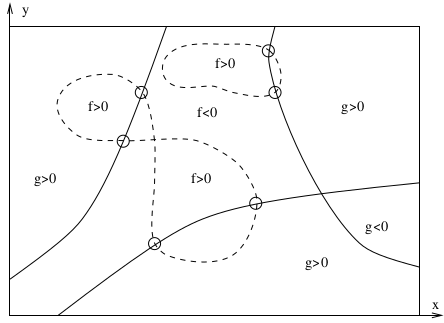
\includegraphics[width=0.75\linewidth]{img/9/9_1.png}
\end{figure}
$$
\left.\begin{array}{l}
f(x,\ y)=0\\
g(x,\ y)=0
\end{array}\right\} 
$$
 \end{frame}
\begin{frame}{Wstęp}
\textbf{Problemy:}
\begin{itemize}
\item kontury zerowe $\rightarrow$ podział płaszczyzny,
\item $\mathrm{f},\mathrm{g}-$dowolne $\Rightarrow$kontury bardzo złożone,
\item {\it liczba zer nie jest znana a priori},
\item dla $ x>2\rightarrow$hiperpłaszczyzny,
\item jak wybrać punkty startowe?
\item kiedy zakończyć poszukiwanie miejsc zerowych?
\item konieczność wyboru rozwiązania, którego poszukujemy $\rightarrow$ nie szukamy wszystkich
\end{itemize}

\textbf{Uwaga:}$\newline$
Wykorzystujemy wiedzę z analizy matematycznej, geometrii, algebry !!!
\end{frame}

\begin{frame}{Wstęp}
\textbf{Przykładowe układy równań nieiniowych - wizualizacja:}
$\newline$
\url{https://www.symbolab.com/solver/non-linear-system-of-equations-calculator}
$\newline$ $\newline$ 
\textbf{Zastosowanie układów równań nieliniowych:}
\begin{itemize}
	\item kinetyka reakcji chemicznych, badanie równowagi termodynamicznej układu, przewidywanie istnienia związków chemicznych
	\item sterowanie elektrycznymi silnikami prądu stałego
	\item badanie dynamiki samolotów (nieliniowe zależności prędkości, kątów,wysokości...)
	\item układy automatyczne, problem utrzymania równowagi w układach niestabilnych - drony
	\item ...
\end{itemize}
\end{frame}
% 	%%%%%%%%%%%%%%%%%%%%%%%
\section{Metoda iteracyjna dla układów równań nieliniowych}

\begin{frame}{Metoda iteracyjna dla układów równań nieliniowych}

  $$\boxed{\overrightarrow{f}(\overrightarrow{x})=0} $$ zapisujemy jako:
  $$x_i=\varphi_i(x_1,x_2,...,x_m) , i=1,2,...,m$$
  co sugeruje metodę iteracyjną:
  $$x_i^{(n)}=\varphi_i(x_1^{(n-1)},x_2^{(n-1)},...,x_m^{(n-1)}) , i=1,2,...,m$$
  $$\boxed{\overrightarrow{x}^{(n)}=\overrightarrow{\varphi}(\overrightarrow{x}^{(n-1)})}\quad(\star)$$
\end{frame}

\begin{frame}{}
  \begin{block}{Kryterium zbieżności}
  	\textbf{Niech:}
    \begin{itemize}
      \item[-] $\overrightarrow{\alpha}=\overrightarrow{\varphi}(\overrightarrow{\alpha})$
      \item[-] istnieją $d_{ij}(\overrightarrow{x})=\frac{\partial\varphi_i(\overrightarrow{x})}{\partial x_j}$ , $i,j=1,2,...,m$\\
      dla $\overrightarrow{x}\in R^m=\{\overrightarrow{x}:||\overrightarrow{x}-\overrightarrow{\alpha}||<\rho\} \Rightarrow$\\
      D-macierz o elementach $d_{ij}$
    \end{itemize}
  \end{block}
\end{frame}

\begin{frame}{}
  \begin{block}{Kryterium zbieżności}
    \emph{Wtedy:}
    \begin{itemize}
      \item[-] \textbf{warunek wystarczający zbieżności ($\star$)} dla $\overrightarrow{x}_0\in R^m$\\
      $$||D(\overrightarrow{x})||\leq L<1\quad,\quad\overrightarrow{x}\in R^m:$$
      ($\varphi$ - \emph{odwzorowanie zwężające} (contraction mapping)\\ $\Rightarrow$ dla dowolnych $\overrightarrow{x},\overrightarrow{y}: ||\overrightarrow{\varphi}(\overrightarrow{x})-\overrightarrow{\varphi}(\overrightarrow{y})||\leq L \cdot ||\overrightarrow{x}-\overrightarrow{y}||)$
      \item[-] \textbf{warunek konieczny zbieżności ($\star$)}\\
      promień spektralny $\rho(D)\leq 1$
      \item \textbf{prędkość zbieżności} - zależna liniowo od L
    \end{itemize}
  \end{block}
\end{frame}
% 	%%%%%%%%%%%%%%%%%%%%%%%
\section{9.3 Metoda Newtona-Raphsona dla układów równań nieliniowych}

\begin{frame}{}
  \begin{itemize}
    \item $\{x_j^{(n-1)}\}$ - przybliżenie pierwiastków $\{\alpha_j\}$
    \item $\alpha_j=x_j^{(n-1)}+h_j$\\
    $f_i(\overrightarrow{x}^{(n-1)}+\overrightarrow{h})=0\quad\rightarrow\quad$szereg Taylora:
    $$f_i(\overrightarrow{x}^{(n-1)})+\sum_{j=1}^{m}(\frac{\partial f_i}{\partial x_j})_{n-1} \cdot h_j+\underbrace{O(\delta x^2)}_{pomijamy}=0\quad(\star\star)$$
    gdzie $(\frac{\partial f_i}{\partial x_j})_{n-1}$- oznacza obliczone w $\overrightarrow{\alpha}^{(n-1)}$
  \end{itemize}
\end{frame}

\begin{frame}{}
  Jako kolejne przybliżenie $\alpha$ bierzemy $\overrightarrow{x}^{(n)}=\overrightarrow{x}^{(n-1)}+\overrightarrow{h}$\\
  przy czym $\overrightarrow{h}$ - wyznaczamy z $(\star\star)$\\
  Można to zapisać:
 $$
 \left.
 \begin{array}{lr}
 J^{(n1)} \cdot \overrightarrow{h}^{(n-1)} = -\overrightarrow{f}^{(n-1)}\\
 \overrightarrow{x}^{(n)} = \overrightarrow{x}^{(n-1)}+\overrightarrow{h}^{(n-1)}
 \end{array}\right\}
 \text{- układ równań liniowych}
 $$
  jakobian:
  $$J^{(n-1)}_{i,j}=(\frac{\partial f_i}{\partial x_i})_{(n-1)}$$
\end{frame}

\begin{frame}{}
  \begin{block}{trudności}
    \begin{itemize}
      \item wybór $\overrightarrow{x}^{(0)}$,
      \item sprawa zbieżności - trudna w przypadku ogólnym,
      \item złożoność obliczeniowa
      \begin{itemize}
        \item[-] $J\leftarrow m^2$ elementów:
        \begin{itemize}
          \item[$\star$] formalnie różniczkowanie,
          \item[$\star$] wprowadzanie do programu
        \end{itemize}
        \item[-] w każdej iteracji - J - na nowo,
        \item[-] h - z rozwiązania układu równań liniowych.
      \end{itemize}
    \end{itemize}
  \end{block}
\end{frame}


% 	%%%%%%%%%%%%%%%%%%%%%%%
\section{Modyfikacje metody N-R dla układów równań nieliniowych}

\begin{frame}{Modyfikacje metody N-R dla układów równań nieliniowych}
  \begin{block}{1) damped iterates}
    $$F^{(n)}=\sum_{i=1}^{m} [f_i^{(n)}]^2$$
    gdy $F^{(n)}<F^{(n-1)}\quad\overrightarrow{x}^{(n)}$ - akceptujemy\\
    w przeciwnym razie $\rightarrow$ próbujemy:
    $$\overrightarrow{x}^{(n)}=\overrightarrow{x}^{(n-1)}+\rho \cdot \overrightarrow{h}^{(n-1)}$$
    $$0<\rho<1,\text{ zwykle kolejno } \rho=\frac{1}{2},\frac{1}{4},\frac{1}{8}$$
  \end{block}
\end{frame}

\begin{frame}{}
  \begin{block}{2)}
    J-duża złożoność obliczeniowa
    $$J^{(n-1)}\text{ używamy dla }p\text{ iteracji:}$$
    $$J^{(n-1)} \cdot \overrightarrow{h}^{(n-1+k)}=-\overrightarrow{f}^{(n-1+k)}$$
    $$\overrightarrow{x}^{(n+k)}=\overrightarrow{x}^{(n-1+k)}\overrightarrow{h}^{(n-1+k)}, k=0,1,...,p-1$$
    dobór $p$?
  \end{block}
\end{frame}

\begin{frame}{}
  \begin{block}{3)}
    $$\overrightarrow{x}^{(n)}=\overrightarrow{x}^{(n-1)}-\underbrace{[J^{(n-1)}]^{-1}}_{(*)}\overrightarrow{f}^{(n-1)}$$
    $$(*)\ H^{(n-1)}-\text{ przez przybliżenie}$$
    $${i:H^{(n)}=H^{(n-1)}+\underbrace{D^{(n-1)}}_{(**)}}$$
    $$(**)\rightarrow\text{ człon korekcyjny}$$
  \end{block}
\end{frame}
% 	%%%%%%%%%%%%%%%%%%%%%%%
\end{document}
